\documentclass[a4paper,10pt]{article}
\fontfamily{book antiqua}
\usepackage{graphicx}
\usepackage{amsmath}
\usepackage{amsfonts}
\usepackage{amssymb}
\textwidth 15cm
\textheight 23cm
%\oddsidemargin -0.0in
\oddsidemargin -6 true pt 

\begin{document}
\begin{titlepage}
\begin{center}

\begin{Huge}PyMorph\end{Huge}\\
\begin{Large}Software for \\Automated Galaxy Morphological Parameter Estimation\end{Large}\\

\begin{large}
%[Python MORphological Parameters Hunter]
\end{large}
\vspace{5cm}
\vspace{0.5cm}
\begin{Large}Vinu Vikram\end{Large}\\
School of Pure \& Applied Physics\\
Mahatma Gandhi University\\
Kottayam, Kerala, India\\
\vspace{0.3cm}
\begin{Large}Yogesh Wadadekar\end{Large}\\
National Centre for Radio Astrophysics\\
Pune, India\\
\vspace{0.3cm}
\begin{Large}Ajit K. Kembhavi \end{Large}\\
Inter-University Centre for Astronomy and Astrophysics (IUCAA)\\
Pune, India
\vspace{5cm}
2008
\end{center}
\end{titlepage}
\tableofcontents
\clearpage
\section{PyMorph}
{\bf PyMorph} is a software pipeline which computes non-parametric and parametric morphological parameters of galaxies. PyMorph uses GALFIT (Peng et. al. 2002) for bulge disk decomposition of galaxy and SExtractor (Bertin et. al. 1996) for determining the initial values. PyMorph uses its own module to calculate Concentration index, Asymmetry, Clumpness, Gini Coefficient, second order moment of the brightest 20\% pixels of galaxies(CASGM). In this section we will explain PyMorph in detail.
\subsection{Dependencies}
\begin{enumerate}
 \item Python 2.4 or greater
 \item Stsci$\_$python (This package includes numpy, pyfits, pyraf)
 \item GALFIT
 \item SExtractor
 \item matplotlib
 \item xpa (optional, if you want to select PSF)
\end{enumerate}

\subsection{Working modes}
The pipeline works in different modes. A short description of the available modes are the following
\begin{enumerate}
 \item Normal Mode : In normal mode, user will be able give two kind of inputs
\begin{itemize}
\item 
a. A large field(s) of galaxies. eg. HST-ACS/WFPC2, SDSS, 2MASS fields
\item
b. Galaxy(ies) in cutout image(s)
\end{itemize}

\item Repeat Mode : The parameter estimation process can be failed due to several reasons. If the user feels that the fitting can be improved by adjusting the initial values or using an efficient mask, this mode can be used. Here the pipeline will run again on the failed galaxies using the user specified parameters and images. %with the experience gained from past.
\item Find and Fit : Generate parameters of objects which satisfy the magnitude range specified by the user.

\item PSF Selection : To select the PSFs from image

\end{enumerate}
\subsection{Pre-Pipeline Procedure}
\begin{enumerate}
 \item 
Run SExtractor on the frame and the resulting file contains the information of all the object in the frame. The output parameters of this catalogue MUST follow a particular order and that can be found in the Appendix. This is recommended, as the PyMorph may keep the sky value at the SExtractor value during the 2D decomposition. So running SExtractor needs care. If PyMorph does not find any SExtractor catalogue it will create one using the default parameters.
\item
Create a catalogue of galaxies for which the user wants to generate the morphological parameters. The possible columns in the catalogue can be seen the Section \ref{cluscat}. If the FindAndFit mode is enabled, then the program will not search for this catalogue.
\item
Create PSF files% either using PyMorph or by some other means.
\item
Edit the config.py which is the configuration file for the pipeline. The parameters in the configuration file are described in the Section \ref{inputp}.
\end{enumerate}

\subsection{Input parameters}
\label{inputp}
\begin{itemize}
\item \textbf{imagefile:} The large image frame.% This image will be used only if the user are decomposing galaxies in a large frame.

\item \textbf{whtfile:} The corresponding rms/weight map of the large frame. If the name contains the string \textit{wht}/\textit{rms} then the program treats it as weight/rms image. If this file is not found the program will skip this step. 

\item \textbf{sex\_cata:} The SExtractor catalogue of all the objects in the frame. If the user provide one SExtractor catalogue, PyMorph uses it. Otherwise it generate using the default SExtractor parameters in the pipeline. One can use the command line option \textit{--edit-conf} to change these parameters according to their images.

\item \textbf{clus\_cata:} The list of all the objects of interest. The possible columns in this file are given in the Section: \ref{cluscat} and each column must have the title. The program needs at least \textit{gal\_id} or \textit{gimg} to run.

\item \textbf{out\_cata:} The name of the output catalogue. Program will make a catalogue of all the galaxies for which the morphological parameters are generated.

\item \textbf{rootname:} Root name. You can give just a blank '' to avoid this. If the program finds \textit{rootname}, it will be appended to all the intermediate files and the name of the galaxy in the result file.

\item \textbf{psfselect:} Since selecting GOOD PSFs from large frames and make a list of them is time consuming, we have added a small utility which will help the user to find the PSF with out spending much time. This can be achieved by using the psfselect parameter. This parameter can take either 0, 1 or 2. The meaning of these are following
\begin{itemize}
\item 0 $=>$ The pipeline will continue with the user given PSFs.
\item 1 $=>$ The pipeline will run only for finding PSFs.
\item 2 $=>$ Find PSFs and run pipeline.
\item[] It is recommended to use \textit{psfselect} = 1 and select PSFs first. After having
 good PSFs, run pipeline with \textit{psfselect} = 0.
\end{itemize}

% \item \textbf{starsize}
% \begin{itemize}
% \item[] The size of the psf image in terms of the semi-major axis of the image. The size of the image will be\textit{ starsize * semi-major axis}
% \end{itemize}
\item \textbf{psflist:} List of PSFs. You can give it either as a list like \textbf{['psf1.fits, 'psf2.fits', etc]} or point to a file which contains the names of PSFs as \textbf{'@psflist.txt}'. The pipeline will select the nearest PSF to the object of interest either using the header information or using the information from its name. In the latter case, the PSF's name should have the form \textbf{ psf\_radec.fits}.
\begin{verbatim}Eg. If the PSF's position is (12:16:43.5, -12:03:12.0) then the 
name should be psf_1216435-1203120.fits.
\end{verbatim}
This convention is used to find the nearest PSF. The pipline will first check whether the mode is \textit{repeat}. If \textit{repeat} is false and if the program fails to find the configuration file, then it will try to find the coordinate information of the galaxy. If the program doesn't find the RA and DEC information of the galaxy, then it chooses the PSF one by one from the list.

\item \textbf{mag\_zero:} Magnitude zero point.

\item \textbf{mask\_reg, thresh\_area, threshold:} Parameters for masking condition. It is explained in the Section \ref{normal}.

\item \textbf{size:} This parameter is a list of five quantities which controls the size and shape of the stamp image of the galaxy. The size parameters are in the order
\begin{verbatim}
size = [resize, varsize, fracrad, square, fixsize]
\end{verbatim}
\begin{itemize}
\item \textit{resize} - This will be used when the user supply a cutout of galaxy and
 wants to resize the image. This particular parameter is useful when
 we have a large number of frames from surveys like
 SDSS.

\item \textit{varsize} - This parameter will be used to find the image
 cutout size. When it is true the size of the image will be decided from the half light radius of the galaxy.

\item \textit{fracrad} -  Size of the cutout image will be\textit{ fracrad} times half light radius of the
 galaxy.

\item \textit{square} - This will decide the shape of the cutout. If it is true, then the cutout will be square otherwise a rectangle.

\item \textit{ fixsize} - If the user wants to make an image of fixed size,
 this keyword will provide the size information.
\end{itemize}

\item \textbf{pixelscale:}
\item \textbf{H0, WM, WV:} Hubble parameter, $\Omega_M$, $\Omega_\Lambda$

\item \textbf{back\_extraction\_radius:} The radius of the background region which will be used to calculate the background asymmetry and background clumpness.

% \item[] \textbf{angle:}
% \begin{itemize}
% \item The angle of rotation for the calculation of asymmetry
% \end{itemize}

\item The following parameters decide the working mode of PyMorph
\begin{itemize}
\item[] \textbf{repeat:} If it is True, repeat the pipeline manually.
\item[] \textbf{galcut:} True, if the input is cutout of galaxies.
\item[] \textbf{decompose:} True, if the user wants to extract the structural parameters.
\item[] \textbf{cas:} True, if user wants to find the CASGM parameters.
\item[] \textbf{findandfit:} True, to run PyMorph for galaxies within some magnitude range.
\item[] \textbf{crashhandler:} If it is True, then the PyMorph will handle the possible crashes during the pipeline process and try to fix those  errors in the next run. %The details can be found in the Section \ref{crash}
\end{itemize}

\item \textbf{components:} The user can decide the components for fitting. By default PyMorph assumes a disk and a bulge to model the light distribution of the galaxy. The available components are bulge, disk and point.
\item \textbf{fitting} This is also a list of three parameters which can be used to fix/fit center and sky.
\begin{verbatim} fitting = [bulge_center, disk_center, sky]
\end{verbatim}
% \item The following parameters are used to classify good/bad fit.
% \begin{itemize}
% \item[] \textbf{chi2sq:}
% \begin{itemize}
% \item Good fit if the Chi2Nu $<$ chi2sq
% \end{itemize}
% 
% \item[] \textbf{Goodness:}
% \begin{itemize}
% \item Good fit if the Goodness $>$ Goodness
% \end{itemize}

\item \textbf{center\_deviation:} Using this parameter, the user can specify the amount of deviation allowed for the center. If the fitted center deviates from the initial center more than this amount, that will be considered as a crash and refit the galaxy, provided the \textit{crashhandler} is True.
% \end{itemize}

\end{itemize}
\subsection{config.py}
Here is the configuration file for PyMorph.
\begin{footnotesize}
\begin{verbatim}
"""Configure file for PyMorph. Authors: Vinu Vikram, Yogesh Wadadekar Ajit Kembhavi"""
###----Specify the input images and Catalogues----###
imagefile = 'j8f643-1-1_drz_sci.fits'
whtfile = 'j8f643-1-1_drz_rms.fits'  #The weight image. 
sex_cata = 'j8f643_sex.cat'          #The sextractor catalogue which has 
                                     #the format given in the file
clus_cata = 'cl1216-1201.cat'        #catalogue of galaxies from
                                     #online catalogue service
                                     #(name ra1 ra2 ra2 dec1 dec2 dec3)

###----Specify the output names of images and catalogues----###
out_cata = 'cl1216-1201_out.cat'     #catalogue of galaxies in the field
rootname = 'j8f643'

###----Psf list----###
psfselect = 0                        #0 => No psfselection
                                     #1 => Only Select psf 
                                     #2 => Select psf and run pipeline
                                     #Recommended: Run with '1' and then run
                                     #pipeline
starsize = 20                        #psf image size will be startsize times 
                                     #the SMA given by SExtractor
#psflist = ['psf_1216382-1200443.fits', 'psf_1216408-1200251.fits']
psflist = '@psflist.list'
                                     #List of psf contains their 
                                     #position information in the 
                                     #header (RA_TARG, DEC_TARG). 
                                     #Make psf with the names as here 
                                     #and use psf_header_update.py. 
                                     #It will update the header information.
mag_zero = 25.256                    #magnitude zero point

###----Conditions for Masking----###
manual_mask = 0
mask_reg = 2.0
thresh_area = 0.2
threshold = 3.0                      #Masking will be done for neighbours 
                                     #whose semimajor*threshold overlaps with 
                                     #threshold * semi-major axis of 
                                     #the object and area of the neighbour 
                                     #less than thresh_area * object area in
                                     #sq.pixel. 
                                     #The masking will be for a circular 
                                     #region of radius mask_reg*semi-major 
                                     #axis of the nighbour with respect to 
                                     #the center of the neightbour.
###---Size of the cut out and search conditions---###
###---size = [resize?, varsize?, fracrad, square?, fixsize]---###
size = [0, 1, 6, 1, 120]             #size of the stamp image
searchrad = '0.3arc'                 #The search radius  

###----Parameters for calculating the physical parameters of galaxy----###
pixelscale = 0.045                   #Pixel scale (arcsec/pixel)
H0 = 71                              #Hubble parameter
WM = 0.27                            #Omega matter
WV = 0.73                            #Omega Lambda

###----Parameters to be set for calculating the CASGM----###
back_extraction_radius = 15.0
#back_ini_xcntr = 32.0 
#back_ini_ycntr = 22.0
angle = 180.0

###----Fitting modes----###
repeat = False                       #Repeat the pipeline manually
galcut = False                       #True if we provide cutouts
decompose = True
galfit = True #Always keep this True as it is not functional yet!
cas = True
findandfit = 0
crashhandler = 1

###---Galfit Controls---###
components = ['bulge', 'disk']       #The components to be fitted to the objec
###---fixing = [bulge_center, disk_center, sky]
fitting = [1, 1, 0]                  # = 0, Fix params at SExtractor value

###----Set the SExtractor and GALFIT path here----###
GALFIT_PATH = '/home/vinu/software/galfit/modified/galfit' 
SEX_PATH = '/home/vinu/software/sextractor-2.5.0/sex/bin/sex'
PYMORPH_PATH = '/home/vinu/serial_pipeline/trunk/pymorph'

###----The following conditions are used to classify fit goo/bad----###
chi2sq = 1.9                         #< chi2sq
Goodness = 0.60                      #> Goodness
center_deviation = 3.0               #< abs(center - fitted center)
\end{verbatim}
\end{footnotesize}
\subsection{Possible columns in clus\_cata}
\label{cluscat}
\begin{itemize}
\item \textbf{ gal\_id:} The identifier of the galaxy.
\item \textbf{ ra1, ra2, ra3:} The RA of the galaxy. ra1 is the degree part, ra2 is minute and ra3
 is the second part.
\item \textbf{ dec1, dec2, dec3:} The DEC of the galaxy and have same syntax as RA
\item \textbf{ z:} The redshift of the galaxy
\item \textbf{ gimg:} The galaxy image if PyMorph runs in GALCUT mode (ie. input will be cutouts of galaxies).
\item \textbf{ wimg:} The corresponding weight image
\item \textbf{ cfile:} Configuration file for GALFIT (if user wants to run PyMorph manually)
\item \textbf{ ximg:} The x center of the galaxy
\item \textbf{ yimg:} The y center of the galaxy
\item \textbf{ bxcntr:} The x center of the background to find the CASGM parameters
\item \textbf{ bycntr:} The y center of the background to find the CASGM parameters
\item \textbf{ psf:} The PSF corresponding to the galaxy
\item \textbf{ flag:} This will be used when the\textit{ crashhandler} is on. See the Flags section to know more.
\end{itemize}

\subsubsection*{Example clus\_cata}
The clus\_cata looks something like the following
\begin{footnotesize}
\begin{verbatim}
gal_id ra1 ra2 ra3 dec1 dec2 dec3 mag z bxcntr bycntr ximg yimg cfile psf flag
EDCSNJ1216453-1201176 12 16 45.26 -12 01 17.6 20.663 0.7955 20.0 20.0 60.0 60.0 
Gj8f647_EDCSNJ1216453-1201176.in psf_1216435-1203120.fits 128
\end{verbatim}
\end{footnotesize}
Another look
\begin{footnotesize}
\begin{verbatim}
gimg wimg ximg yimg bxcntr bycntr
Ij8f647_EDCSNJ1216453-1201176.fits Wj8f647_EDCSNJ1216453-1201176.fits 60.0 60.0 20.0 20.0
\end{verbatim}
\end{footnotesize}
The minimal clus\_cata
\begin{footnotesize}
\begin{verbatim}
gimg
Ij8f647_EDCSNJ1216453-1201176.fits
\end{verbatim}
\end{footnotesize}
Here we assumed that the image \textit{Ij8f647\_EDCSNJ1216453-1201176.fit}s contains a galaxy within 10 pixels
 radius from the center. In the case of cutouts, the minimal configuration which uses all the PyMorph functionalities is the following
\begin{footnotesize}
\begin{verbatim}
gimg z
Ij8f647_EDCSNJ1216453-1201176.fits 0.79
\end{verbatim}
\end{footnotesize}
\subsection{Command line Options}
Some command line options are also available and are explained as follows
\begin{itemize}
 \item 
\textbf{ --edit-conf (-e):} PyMorph uses default set of parameters to generate SExtractor catalogue. These parameters can affect the photometric output from SExtractor. This option allows the user to edit the SExtractor configuration file interactively.

\item
\textbf{ --force (-f): } Normally PyMorph will not generate SExtractor catalogue if it find one. Using this option user can force the pipeline to generate SExtractor catalogue.
\item
\textbf{ --with-psf: } By default, PyMorph will use the nearest PSF from the psflist during decomposition. User can alter this behavior by this parameter. So \textit{--with-psf=0} takes the nearest PSF, \textit{--with-psf=1} uses second nearest PSF and so on. By using \textit{--with-psf=-1} one can select the farthest available PSF. This option becomes  important when the user wants to test the results with different PSFs in the frame.
\item
\textbf{ --help (-h): } 
\item
\textbf{ --lmag}, \textbf{ --umag:} Magnitude constraints for GALFIT.
\item
\textbf{ --ln}, \textbf{ --un: } The minimum and maximum allowed values of Se\'rsic index. Defaults are 0.1 and 20.0.
\item
\textbf{ --lre},\textbf{ --ure: } Minimum and maximum allowed values of bulge scale length, re. Default 0 and 500 pixels.
\item
\textbf{ --lrd},\textbf{ --urd: } Minimum and maximum allowed values of disk scale length, rd. Default 0 and 500 pixels.
\item
\textbf{ --with-in: } Fitting will be done for objects which are NXPTS / 2 + \textit{with-in} or NYPTS / 2 + \textit{with-in} from the main object. By default it takes a value of 150. Usage: \textit{--with-in=150}.
\textbf{ --with-filter:} Manually give the filter. This will go to the database.
\textbf{ --with-db:} The MySQL database name.
\textbf{ --with-area:} The area of PSFs.
\end{itemize}

\subsection{Working}
The architecture of the PyMorph is shown in the Figures \ref{fig:arch1}, \ref{fig:arch2} and explained as follows

 \begin{figure}%[tbh!]
 \centering
 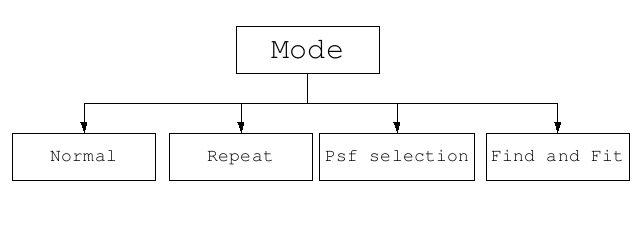
\includegraphics[width=8cm, height=3.5cm, bb=0 0 641 234]{pipeline-arch1.png}
 % pipeline-arch1.png: 641x234 pixel, 72dpi, 22.61x8.26 cm, bb=0 0 641 234
 \caption{The PyMorph Modes}
 \label{fig:arch1}
\end{figure}

 \begin{figure}%[tbh!]
 \centering
 \includegraphics[scale=0.5]{pipeline-full.png}
 % pipeline-arch1.png: 641x234 pixel, 72dpi, 22.61x8.26 cm, bb=0 0 641 234
 \caption{The PyMorph Architecture}
 \label{fig:arch2}
\end{figure}

% \begin{figure}[tbh!]
%  \centering
%  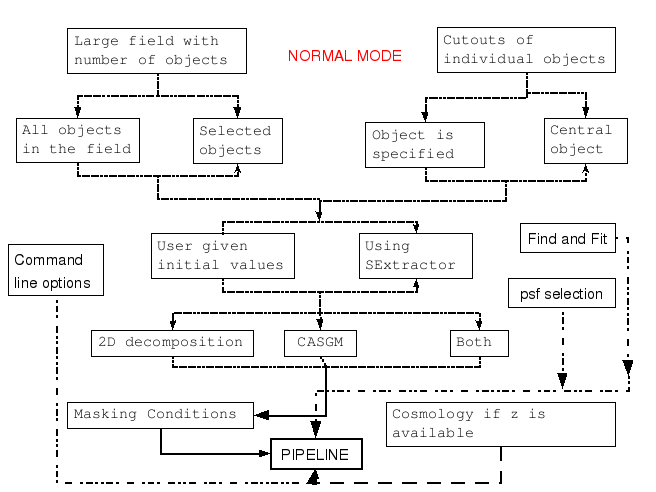
\includegraphics[width=11cm, height=8.5cm, bb=0 0 656 492]{pipeline-arch2.png}
%  % pipeline-arch2.png: 656x492 pixel, 72dpi, 23.14x17.36 cm, bb=0 0 656 492
%  \caption{PyMorph Architecture}
%  \label{fig:arch2}
% \end{figure}
% 
% \begin{figure}[tbh!]
%  \centering
%  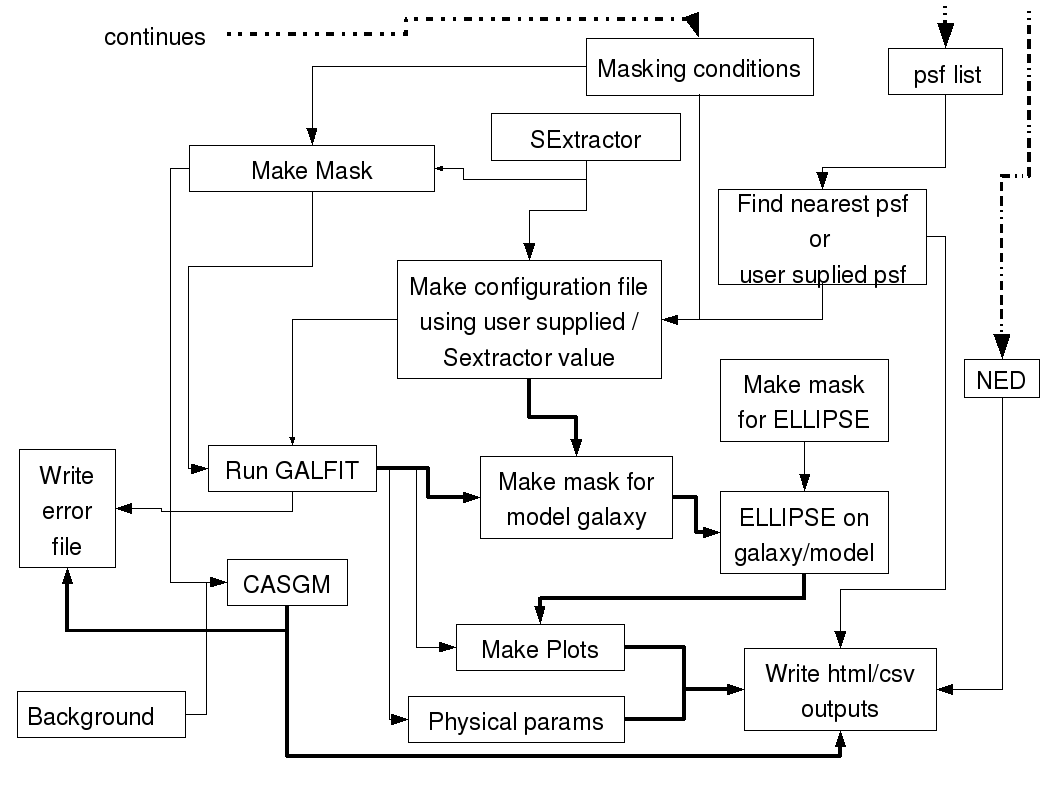
\includegraphics[width=11cm, height=8.5cm, bb=0 0 794 596]{pipeline-arch3.png}
%  % pipeline-arch3.png: 1058x794 pixel, 96dpi, 28.00x21.01 cm, bb=0 0 794 596
%  \caption{PyMorph Architecture}
%  \label{fig:arch3}
% \end{figure}
% 
% \begin{figure}[tbh!]
%  \centering
%  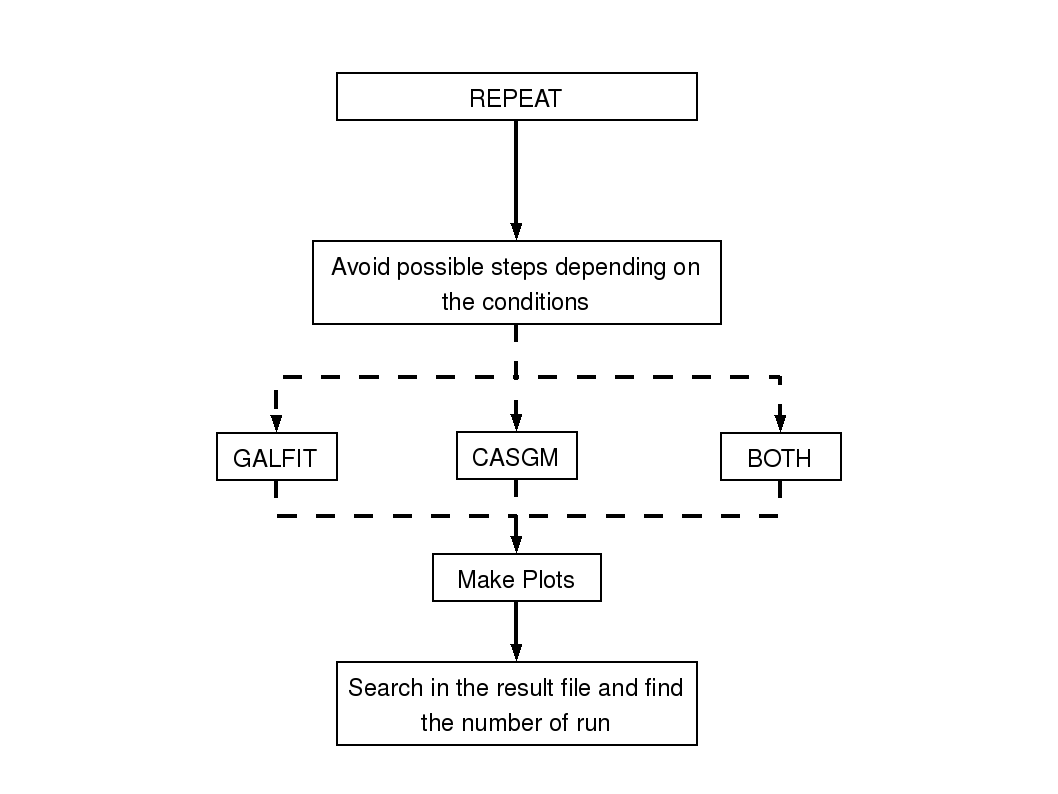
\includegraphics[width=11cm, height=8.5cm, bb=0 0 794 596]{pipeline-arch4.png}
%  % pipeline-arch4.png: 1058x794 pixel, 96dpi, 28.00x21.01 cm, bb=0 0 794 596
%  \caption{PyMorph Repeat Mode}
%  \label{fig:arch4}
% \end{figure}


\subsubsection{Normal Mode with large field}
\label{normal}
PyMorph compares the user given galaxy catalogue (\textit{clus\_cata}) and SExtractor catalogue (\textit{sex\_cata}). If the pipeline finds an object in the SExtractor catalogue, it will create a stamp image and the corresponding weight map of the galaxy. Initially the pipeline try to match the RA and DEC information from the \textit{clus\_cata} with SExtractor catalogue using \textit{serachrad}. If the \textit{clus\_cata} doesn't have RA, DEC information the pipeline will try to compare it with the pixel coordinate of the object in the frame. For that it will search for columns with headers \textit{ximg} and \textit{yimg}. The pipeline stops if it does not find these columns. To find the structural parameters the pipeline works as follows.

The first step in 2D bulge-disk decomposition is the creation of stamp size image of the object. 
The size of the image should be in such a way that the image must include enough sky and should not loose light from the outer part of the objects.
An image with very large size will leads to the unnecessary usage of CPU.
We use the FLUX\_RADIUS ($R_{50}$), THETA\_IMAGE ($\theta$), ELONGATION ($\frac{a}{b}$) values from SExtractor to find the required size of the cutout.
Here the FLUX\_RADIUS corresponds to the half light radius ($R_{50}$) of the galaxy.
The size of the stamp image will be found by the following formula
\begin{equation}
X = F_{\textrm{rad}} R_{50} \left(|\cos\theta| + \frac{b}{a} | \sin\theta |\right)
\end{equation}
\begin{equation}
Y = F_{\textrm{rad}} R_{50} \left(| \sin\theta | + \frac{b}{a} | \cos\theta |\right)
\end{equation}
where X and Y are the x and y dimension of the stamp image. 
$F_{rad}$ is the user specified controlling parameters.
In our case we found $F_{rad} = 6$ is a good compromising value for the determination of the postage stamp.
We cut same portion of the noise map and use it as the weight image to GALFIT.

GALFIT allows us to fit more than one objects simultaneously.
We fit a single Se\'rsic function to the neighbour objects to reduce the contamination from these objects to the main galaxy.
So the next step is to find the neighbour objects and determine whether it should be fitted simultaneously with the main object.
To do that, we use SExtractor A\_IMAGE (R) and ISO0 (A) parameters of both objects and neighbour.
The criterion for simultaneous fit is the following
\begin{eqnarray}
|x_o - x_n| &<& T_R (R_o + R_n) \quad \textrm{or} \nonumber \\
|y_o - y_n| &<& T_R (R_o + R_n) \quad \textrm{or} \nonumber \\
A_n &>& T_A A_o 
\label{sim-fit}
\end{eqnarray}
where $x_o$, $x_n$, $y_o$, $x_n$ are the x and y centers of object and neighbour and $R_o$, $R_n$, $A_o$ and $A_n$ are the A\_IMAGE and ISO0 of object and neighbour. 
We found the controlling parameters $T_R = 3.0$ and $T_A = 0.3$ are promising.
We mask all the neighbour objects which does not satisfy the above criterion (Eqn \ref{sim-fit}).
We mask all the pixels of the neighbour objects which satisfy $r < T_M R_n$, where r is the radius in an elliptical aperture. 
We have used $T_M = 2.0$ so that all the pixels of the neighbour object will be masked.
This masking technique will work only if SExtractor detect the neighbour object. 
Since the detection depends on the DETECT\_THRESH and DETECT\_MINAREA parameters, it is possible that some furious pixels can left undetected by SExtractor.
So we use the following simple technique to mask those furious pixels.
From the center of the main object we make elliptical annuli with increasing radii.
In the inner aperture we find the maximum value of the galaxy.
We assume a smooth distribution for the galaxy's light profile which decreases from the center.
This implies the largest value in the central elliptical aperture is the maximum value the object can have.
So we mask all the other pixels outside the inner aperture with value greater than this maximum value.
Now we go to next annulus and find the maximum and mask other pixels outside this aperture which has value larger than the maximum of this aperture.
This procedure continue till the aperture radius hit the image limit.
Then we use a set of binary morphology operations to clean the mask.
Now almost all the furious pixels and undetected objects will be masked properly and we combine this with the neighbour mask.

Next step is to find initial values for the fitting parameters.
To each galaxy in the catalogue we fit a Se\'rsic and exponential functions.
The Se\'rsic function which is used to model the luminosity profile of the bulge part is given by
\begin{equation}
 I(r) = I_e e^{-b_n (\frac{r}{r_e}^{1/n} - 1)}
\end{equation}
 and the exponential function which model the disk part of the galaxy is given by
\begin{equation}
 I(r) = I_d e^{-\frac{r}{r_d}}
\end{equation}
where $r_e$ is the bulge scale length, $n$ is the Se\'rsic index and $r_d$ is the disk scale length. $b_n$ is a parameter which depends on the Se\'rsic index.

GALFIT accepts the initial values of the total magnitude, scale radii, axis ratios and position angles of bulge and disk and Se\'rsic index of the bulge.
We set MAG\_AUTO value from SExtractor as the input value to the total magnitudes of both bulge and disk.
For the scale radii we give the half light radius of the galaxy.
By default PyMorph set the initial value for Se\'rsic index (n) to 4, which corresponds to de Vaucouleurs' law.
After setting the initial value we create a contrain file, which restrict the free parameters from going to unphysical values during the fit.
The position angle and axis ratio are set from the values of the THETA\_IMAGE and ELONGATION parameters.

The estimation of CASGM parameters are explained in the Section \ref{casgm}. Finally the pipeline creates diagnostic plots (Figures 3, 4) and results in different formats which includes html, csv, mysql database and fits cutouts.
\begin{figure}
 \centering
 \includegraphics[scale=0.5]{P_Ij8f648_EDCSNJ1216446-1201089.png}
 % P_Ij8f648_EDCSNJ1216446-1201089.png: 666x402 pixel, 72dpi, 23.49x14.18 cm, bb=0 0 666 402
 \label{fig:output}
\caption{Output image from PyMorph}
\end{figure}

\begin{figure}
 \centering
 \includegraphics[scale=0.3]{pymorph-html.jpg}
 % P_Ij8f648_EDCSNJ1216446-1201089.png: 666x402 pixel, 72dpi, 23.49x14.18 cm, bb=0 0 666 402
 \label{fig:html}
\caption{HTML output from PyMorph}
\end{figure}
\subsubsection{Normal Mode with cutouts}
 In this mode the pipeline follows the same route as explained in the previous section. In this case if the program doesn't find the RA, DEC information or the centroid of the object, it extract the morphological parameters of the object in the center of the image. 
\subsubsection{Repeat Mode}
During this mode of run the pipeline will not create or modify the mask image or GALFIT configuration file, if they exist. So one can adjust his GALFIT configuration file / mask image before running the pipeline in the REPEAT mode.
\subsubsection{Find and Fit}
In this mode user can fit objects without creating \textit{clus\_cata}. The user has to give the magnitude range of the object to be fitted. This is useful when one wants to find the quantitative morphology of all the objects in the frame. 
% \subsubsection{Psf Selection}
% One of most difficult problem during the Morphological parameter estimation is to get good psf. Even in the case of PyMorph the situation won't differ much. But PyMorph is providing a very handy tool to select the psf out of the frame. As one the collaborator tells, this procedure is something like playing computer game. It is interesting but need much care. The keywords in config.py, \textit{'psfselect'} and \textit{'starsize'} are the controlling parameters of the mode. By default PyMorph will find the nearest psf from the psf list. This will cause some problem while you are using cut image, where you will have one psf corresponding to one galaxy. Taking this in to account PyMorph will update the clus\_cata with one psf to each galaxy under the column \textit{'psf'}.
% \subsubsection{Crash Handler}
% \label{crash}
% If the parameter \textit{crashhandler} is on in the config.py, it will be invoked in three situations
% \begin{itemize}
% \item Galfit crashes or one of the bulge / disk parameter hits the limit
% \begin{itemize}
% \item[] Solution: Try to fit again with the following conditions
% \begin{itemize}
% \item Fix / free sky, if it is free / fix
% \item Fix / free centers of bulge and disk, if the centers are found free / fix
% \end{itemize}
% \end{itemize}
% 
% \item Reduced chi square is large
% \begin{itemize}
% \item[] Solution: Fix / free centers of bulge and disk, if the centers are found free / fix
% \end{itemize}
% 
% \item Fake center
% \begin{itemize}
% \item[] Solution: Fix centers of bulge and disk.
% \end{itemize}
% \end{itemize}
% The schematic diagram of crash handle is as following
% \begin{figure}
%  \centering
%  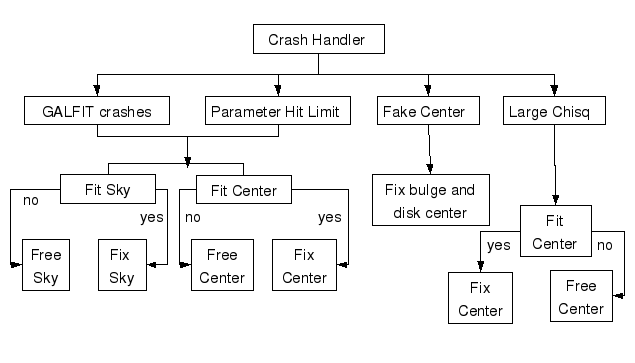
\includegraphics[width=10cm, height=5.7cm, bb=0 0 635 363]{pipeline-arch5.png}
%  % pipeline-arch5.png: 635x363 pixel, 72dpi, 22.40x12.81 cm, bb=0 0 635 363
%  \caption{Crash Handler}
%  \label{fig:arch5}
% \end{figure}

\subsection{Filenames}
The PyMorph makes a number of files and those filenames follow unique format. The filename convention is illustrated below. Suppose in the config.py the parameter \textit{rootname} = j8f645 and \textit{gal\_id}, which is the name of the galaxy in the \textit{clus\_cata} is 9999, then
\begin{itemize}
\item \textbf{Ij8f645\_9999.fits:} The cut out of the galaxy.
\item \textbf{Wj8f645\_9999.fits:} Corresponding weight image.
\item \textbf{Mj8f645\_9999.fits:} Mask image for GALFIT.
\item \textbf{EMj8f645\_9999.fits:} Mask image for ellipse fitting.
\item \textbf{EMj8f645\_9999.fits.p:l} EMj8f645\_9999.fits will be converted to EMj8f645\_9999.fits.pl for
 ellipse task.
\item \textbf{Gj8f645\_9999.in:} Configuration file for GALFIT.
\item \textbf{Oj8f645\_9999.fits:} The output image from GALFIT.
\item \textbf{fit2.log:} The output parameters will be append to this file
\item \textbf{error.log:} The status of the process. From this file the user gets the information about crashes.
\item \textbf{E\_j8f645\_9999.txt:} 1D surface brightness profile of the input image.
\item \textbf{OE\_j8f645\_9999.txt:} 1D surface brightness profile of the model.
\item \textbf{P\_j8f645\_9999.png:} The plot of input, output, residue images and the 1-D profile comparison.
\item \textbf{R\_j8f645\_9999.html:} The html output.
\item \textbf{index.html:} The index file of all the objects.
\item \textbf{result.csv:} The csv file contains all the parameters
\item \textbf{agm\_result\_with\_radius.csv:} The file contains the radial variation of Asymmetry , Gini coefficients and M20. Also $r_{20}$, $r_{50}$, $r_{80}$, $r_{90}$, Petrosian radius etc. are included.
\item \textbf{restart.cat:} The catalogue contains all the failed objects with the corresponding lines in the \textit{clus\_cata}. This catalogue can be used to restart the PyMorph in the case of failed galaxies.
\item \textbf{CRASH.CAT:} Probably the user may not want to use this. This will be used by the pipeline if the \textit{crashhandler} is True.
\end{itemize}

\section{CASGM Module}
\label{casgm}
 Concentration, Asymmetry, Clumpness, Gini coefficient and Moment of the galaxy (CASGM) are widely used to generate quantitative galaxy morphology, for the last few years. %(Abraham et. al. 1996; Bershady et. al., Conselice et. al. 2003; Lotz et. al. 2004). 
In this section we describe the implementation of these parameters in \textbf{PyMorph}.

\subsection{Concentration (C)}

1. Find the Petrosian radius $r_{\eta}$ at which parameter ($\eta$) becomes 0.2. The Petrosian parameter, $\eta$,  is defined as 
\begin{equation}
\eta = \frac{L(R)}{L(<R)}
\end{equation}

L(R) is the average surface brightness at the radius R and $L(<R)$ is the average brightness inside the radius R.

\begin{figure}[h]
\begin{center}
$\begin{array}{c@{\hspace{1cm}}c}
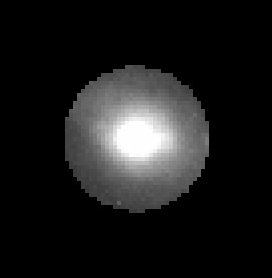
\includegraphics[width=4.5cm,height=4.5cm,bb=0 0 272 278]{C_r20.jpg}&
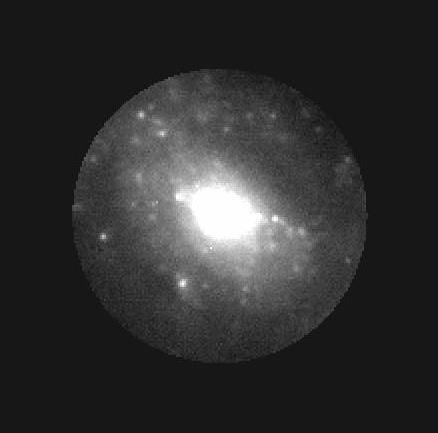
\includegraphics[width=4.5cm,height=4.5cm,bb=0 0 438 433]{C_r80.jpg}\\[0.1cm]
\mbox{20\% light contained portion} & \mbox{80\% light contained portion}
\end{array}$
\end{center}
\caption{Portion of galaxy within $r_{20}$ and $r_{80}$ }% \protect\ref{C and A}}
\label{concentration}
\end{figure}

2. Find the total light of the galaxy as the light inside $1.5 \times r_{\eta}$.

3. Find the $80\%$ and $20\%$ light contained radii. ie. $r_{80}$ and  $r_{20}$.

4. The concentration index will be found using the equation
\begin{equation}
C= 5 \log(\frac{r_{80}}{r_{20}})
\end{equation}

%\vspace{3cm}
\subsection{Asymmetry (A)}

1. Define an extraction region of radius $1.5 \times r_{\eta}$.

2. Rotate the image \footnote{The image used here is of NGC 5585 in R band.} by $180^0$

3. Find the asymmetry parameter using the equation
\begin{equation}
A = \frac{\sum\left|I_0 - I_\phi\right|}{2\sum |I_\phi|}
\end{equation}
where $I_\phi$ is the rotated image and $I_0$ is the original image.

4. Centering correction will be applied by minimizing the A value w.r.t. center.

5. Noise correction will also be done by subtracting the asymmetry of the background from the image asymmetry.


\begin{figure}[h]
\begin{center}
$\begin{array}{c@{\hspace{1cm}}c@{\hspace{1cm}}c}
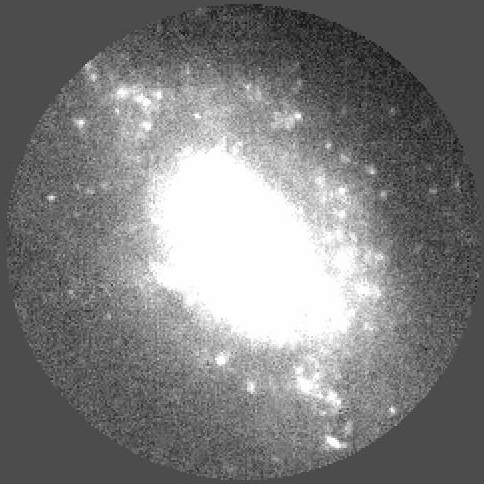
\includegraphics[width=4cm,height=4cm,bb=0 0 484 484]{original.jpg}&
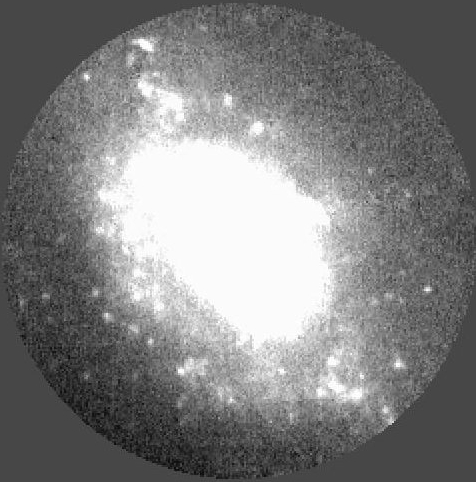
\includegraphics[width=4cm,height=4cm,bb=0 0 476 482]{rotated.jpg}&
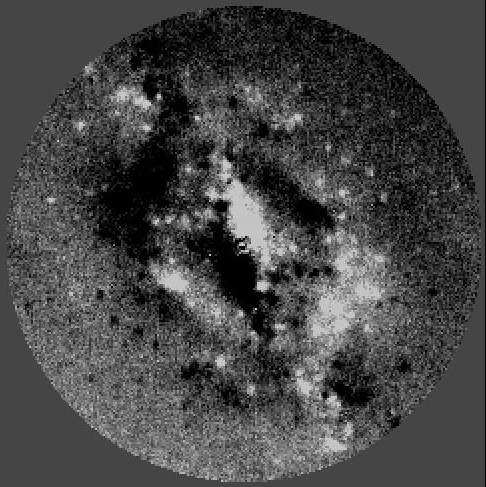
\includegraphics[width=4cm,height=4cm,bb=0 0 486 487]{residue.jpg}\\[0.1cm]
\mbox{Original image} & \mbox{Rotated image} & \mbox{Residual image}
\end{array}$
\end{center}
\caption{Images within the extraction radius}% \protect\ref{C and A}}
\label{Original and Rotated}
\end{figure}

\subsection{Clumpness (S)}

1. Smooth the image with a boxcar of size $r_{\eta}/4$

2. Remove the center region of the galaxy within a radius $r_{\eta}/4$ as the center is not always resolved.

3. Clumpness parameter can be computed using the equation
\begin{equation}
S = 10\times \frac{I - I^\sigma}{I}
\end{equation}

where I is the original image and $I^\sigma$ is the smoothed image.

4. Subtract the background clumpness to get the final clumpness.

\begin{figure}[h]
\begin{center}
$\begin{array}{c@{\hspace{1cm}}c@{\hspace{1cm}}c}
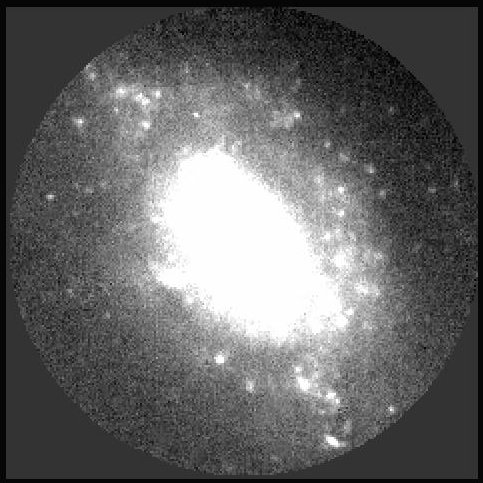
\includegraphics[width=4cm,height=4cm,bb=0 0 483 483]{ori_S.jpg}&
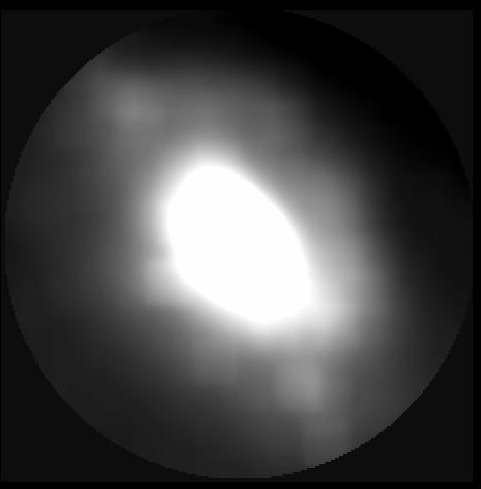
\includegraphics[width=4cm,height=4cm,bb=0 0 481 489]{smoothed.jpg}&
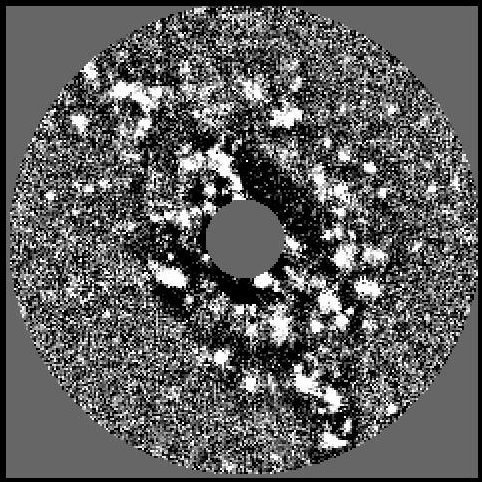
\includegraphics[width=4cm,height=4cm,bb=0 0 482 482]{res_S.jpg}\\[0.1cm]
\mbox{Original image} & \mbox{Smoothed image} & \mbox{Residual image}
\end{array}$
\end{center}
\caption{Images within the extraction radius}% \protect\ref{C and A}}
\label{Original Smoothed and Residual}
\end{figure}

\subsection{Gini coefficient (G)}
Gini coefficient quantifies galaxy's light distribution among the pixels. Its value lie in between 0 and 1. If all the light is concentrated in one pixel, then G will be 1 and if the light distributed uniformly among the pixels, then G will be zero. To find Gini coefficient we use the following technique

1. Create a segmentation map, ie, find the pixels belong to the galaxy. To do this we smooth the image by a boxcar of size $r_{\eta}/5$. This will increase the signal-to-noise ratio at the outer regions of the galaxy. The surface brightness $\mu_{\eta}$ at $r_{\eta}$ is measured and pixels in the smoothed image with flux values greater than $\mu_{\eta}$ and less than $10 \sigma$ is assigned to the galaxy. $\sigma$ is the sky deviation in the image. The upper limit assures that any remaining cosmic rays or spurious noise pixels in the image are not included in the segmentation map.

2. Sort the pixels in the segmentation map according to their photon counts and the Gini coefficient will be computed using the equation
\begin{equation}
G = \frac{1}{\overline{X} n (n-1)}\sum_{i}^n(2i-n-1)X_i
\end{equation}

\begin{figure}[h]
        \centering
        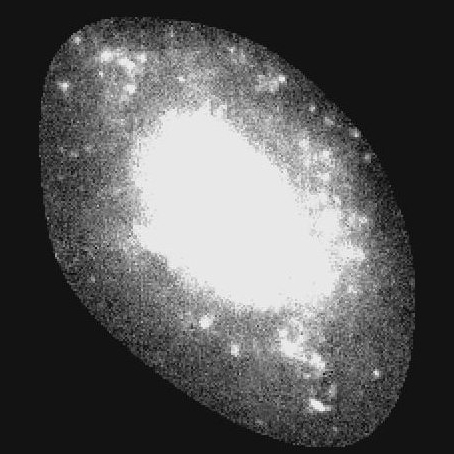
\includegraphics[width=4cm,height=4cm,bb=0 0 454 454]{segmentation.jpg}
% segmentation.jpg: 72dpi, width=22.54cm, height=16.97cm, bb=0 0 639 481
        \caption{Segmentation map of the galaxy}
        \label{fig:9}
\end{figure}

\subsection{The Moment of the Light (M20)}
$M_{20}$ is the second order moment of the brightest $20\%$ pixels of the galaxy.

1. Find the second-order moment $M_{tot}$ of the galaxy. Here only the pixels belongs to segmentation map will be considered. We use the following equation to find $M_{tot}$
\begin{equation}
M_{tot}=\sum_{i}^n M_i=\sum_{i}^n f_i\left[ (x_i-x_c)^2 +(y_i-y_c)^2\right]
\end{equation}

where $x_c, y_c$ is the galaxy's center.

2. Minimize $M_{tot}$ w.r.t. center of the galaxy.

3. Sort the pixels by flux, sum $M_i$ over the brightest pixels until the sum of the pixel values equals $20\%$  of the total galaxy flux, and then normalize by $M_{tot}$.
\begin{equation}
M_20 = \log\left( \frac{\sum M_i}{M_{tot}}\right)
\end{equation}

while $\sum_i f_i <0.2 f_{tot}$

where $f_{tot}$ is the total flux of the segmentation map. The normalization by $M_{tot}$ removes the dependence  on total galaxy flux or size.

\section{Parallel PyMorph}
We have parallelized the pipeline based on Single Program, Multiple Data technique. The algorithm used here is shown in the Figure \ref{fig:para}. In this implementation we will have a master processor and $N_P$ slaves. The master will do the pre-processing and post-processing. In the pre-processing part the master processor will create stamp image of the galaxy and pass it to the slave. This process continues until the number of jobs ($N_J$) less than $N_P$. The slave runs PyMorph in the GALCUT mode and send the result to the master. As soon as the master get the result from the $N^{th}$ slave it creates cutout of another galaxy and send to the same processor. Finally, the master generate a final result file which is the only post-processing part. We have tested the parallel PyMorph and found that if we increase the number of slaves 10 fold, then the time requires to generate the parameters decreases $\sim$ 6 fold.
\begin{figure}
 \centering
 \includegraphics[scale=0.6]{parallel-dia.png}
 % parallel-dia.png: 630x400 pixel, 72dpi, 22.23x14.11 cm, bb=0 0 630 400
 \label{fig:para}
\caption{The schematic diagram of Parallel PyMorph. $N_P$ is the number of slaves and $N_J$ is the number of jobs}
\end{figure}

% \section{Methods}
% \subsection{Masking}
% In PyMorph masking will be done separately for ellipse task and for decomposition. In the case of ellipse task all the neighbors are masked using the SExtractor information. But SExtractor can be failed to resolve small objects near the brighter ones. In that case the PyMorph will try to find those using the following method.
% \begin{itemize}
% \item It will find the maximum value inside a small radius of the object
%  of our interest.
% \item It will search any other pixels out side the small radius above the
%  maximum. If there are something it will mask mask those pixels. Then
%  using that mask, the image will be masked. The central part where the
%  maximum is found will also be masked. Then the radius will be increased
%  further and again find the maximum inside that. This will continue till
%  the image boundary.
% \item If it doesn't find any pixels above the maximum, the program will
%  increase the radius and go on.
% \item After it reaches the image boundary, using the\textbf{ ndimage}\textit{
%  fill\_hole} and\textit{ erosion} functions suitable operations on
%  masking will be done. This will remove one pixel mask etc. In the case
%  of masking for decomposition, only object which doesn't fit will be
%  masked.
% \end{itemize}
% 
% 
% \subsection{Sky Sigma and Background region}
% If the user supply the background center, PyMorph will find the sky deviation from that region. But if these
%  parameters are not given, then the Pymorph will calculate the sky deviation first and then using this find the background region. To find the sky deviation, the PyMorph will first mask all the object detected in the cutout. Then
%  using that mask find the sky deviation. Since the estimation of CASGM parameters needs to know a background region of size \textit{back\_extraction\_radius} defined in the config.py. So the process is as follows
% \begin{itemize}
% \item Take an initial point ($\frac{back\_extraction\_radius}{2}$, $\frac{back\_extraction\_radius}{2}$) in the image.
% \item Find the sky deviation within a region of radius \textit{back\_extraction\_radius}. If this deviation is less than the n * sky sigma (where n = 2 as starting value), take that region as background region, else go to the point ($\frac{back\_extraction\_radius}{2} + 2.0$, $\frac{back\_extraction\_radius}{2} + 2.0$).
% \item The above process will go on till it reaches ($size - \frac{back\_extraction\_radius}{2}$ , $size - \frac{back\_extraction\_radius}{2}$) where size is the image size.
% \item Still the result is negative, increase n from 2 to 3 and continue the process till we find the background region.
% \item This process has disadvantage as it won't consider the gradient of sky.
% \end{itemize}
% \subsection*{Goodness}
% It is defined as the ratio of number pixels within n times sky sigma around sky value to the total number of pixels.

\section{Appendix}
SExtractor needs a configuration file, output parameters file, convolution kernel file and Neural Network file for Star/Galaxy classification files for its execution. 
PyMorph uses the following files as default.
\subsection{SExtractor Configuration File}
\begin{footnotesize}
\begin{verbatim}
#-------------------------------- Catalog ------------------------------------
 
CATALOG_NAME     j8f631_sex.cat       # name of the output catalog
CATALOG_TYPE     ASCII_HEAD     # NONE,ASCII,ASCII_HEAD, ASCII_SKYCAT,
                                # ASCII_VOTABLE, FITS_1.0 or FITS_LDAC
PARAMETERS_NAME  default.param  # name of the file containing catalog contents
 
#------------------------------- Extraction ----------------------------------
 
DETECT_TYPE      CCD            # CCD (linear) or PHOTO (with gamma correction)
DETECT_MINAREA   6              # minimum number of pixels above threshold
DETECT_THRESH    1.5            # <sigmas> or <threshold>,<ZP> in mag.arcsec-2
ANALYSIS_THRESH  1.5            # <sigmas> or <threshold>,<ZP> in mag.arcsec-2
 
FILTER           Y              # apply filter for detection (Y or N)?
FILTER_NAME      default.conv   # name of the file containing the filter
 
DEBLEND_NTHRESH  32             # Number of deblending sub-thresholds
DEBLEND_MINCONT  0.005          # Minimum contrast parameter for deblending
 
CLEAN            Y              # Clean spurious detections? (Y or N)?
CLEAN_PARAM      1.0            # Cleaning efficiency
 
MASK_TYPE        CORRECT        # type of detection MASKing: can be one of
                                # NONE, BLANK or CORRECT
 
#------------------------------ Photometry -----------------------------------
 
PHOT_APERTURES   5              # MAG_APER aperture diameter(s) in pixels
PHOT_AUTOPARAMS  2.5, 3.5       # MAG_AUTO parameters: <Kron_fact>,<min_radius>
PHOT_PETROPARAMS 2.0, 3.5       # MAG_PETRO parameters: <Petrosian_fact>,
                                # <min_radius>
PHOT_FLUXFRAC    0.5            # flux fraction[s] used for FLUX_RADIUS
SATUR_LEVEL      100000.0        # level (in ADUs) at which arises saturation
MAG_ZEROPOINT    25.256            # magnitude zero-point
MAG_GAMMA        4.0            # gamma of emulsion (for photographic scans)
GAIN             1.0            # detector gain in e-/ADU
PIXEL_SCALE      0            # size of pixel in arcsec (0=use FITS WCS info)
 
#------------------------- Star/Galaxy Separation ----------------------------
 
SEEING_FWHM      0.11            # stellar FWHM in arcsec
STARNNW_NAME     default.nnw    # Neural-Network_Weight table filename
 
#------------------------------ Background -----------------------------------
 
BACK_SIZE        64             # Background mesh: <size> or <width>,<height>
BACK_FILTERSIZE  3              # Background filter: <size> or <width>,<height>
 
BACKPHOTO_TYPE   GLOBAL         # can be GLOBAL or LOCAL
 
#--------------------- Memory (change with caution!) -------------------------
 
MEMORY_OBJSTACK  3000           # number of objects in stack
MEMORY_PIXSTACK  300000         # number of pixels in stack
MEMORY_BUFSIZE   1024           # number of lines in buffer
 
#----------------------------- Miscellaneous ---------------------------------
 
VERBOSE_TYPE     NORMAL         # can be QUIET, NORMAL or FULL
WRITE_XML        N              # Write XML file (Y/N)?
XML_NAME         sex.xml        # Filename for XML output

#------------------------------ Check Image ----------------------------------

CHECKIMAGE_TYPE  APERTURES           # can be NONE, BACKGROUND, BACKGROUND_RMS,
                                # MINIBACKGROUND, MINIBACK_RMS, -BACKGROUND,
                                # FILTERED, OBJECTS, -OBJECTS, SEGMENTATION,
                                # or APERTURES
CHECKIMAGE_NAME  check.fits     # Filename for the check-image

#-------------------------------- WEIGHTing ----------------------------------

WEIGHT_TYPE      MAP_RMS           # type of WEIGHTing: NONE, BACKGROUND,
                                # MAP_RMS, MAP_VAR or MAP_WEIGHT
WEIGHT_IMAGE     j8f631_drz_rms.fits    # weight-map filename
WEIGHT_GAIN      N              # modulate gain (E/ADU) with weights? (Y/N)
\end{verbatim}
\end{footnotesize}
\subsection{SExtractor Output Parameters}
\begin{footnotesize}
\begin{verbatim}
NUMBER
X_IMAGE
Y_IMAGE
ALPHA_SKY
DELTA_SKY
FLUX_ISO
FLUXERR_ISO
MAG_ISO
MAGERR_ISO
FLUX_RADIUS
BACKGROUND
THETA_IMAGE
ELONGATION
ISO0
A_IMAGE
FLAGS
CLASS_STAR
MAG_BEST           Uses in the case of findandfit mode
\end{verbatim}
\end{footnotesize}
\subsection{SExtractor Convolution Kernel}
\begin{footnotesize}
\begin{verbatim}
By default PyMorph uses 5x5 convolution mask of a Gaussian PSF with FWHM = 2.5 pixels.
\end{verbatim}
\end{footnotesize}
\subsection{SExtractor Neural Netwrok File}
\begin{footnotesize}
\begin{verbatim}
PyMorph uses the default.nnw file coming with SExtractor
\end{verbatim}
\end{footnotesize}
\subsection{PyMorph Flags}
The flags used in PyMorph are the following

\begin{center}
% use packages: array
\begin{tabular}{ll}
Flag & Explanation \\ 
1 & Repeat Mode \\ 
2 & Fit bulge center \\ 
4 & Fit disk center \\ 
8 & Fit sky \\ 
16 & The cutimage extend goes outside the image \\ 
32 & Galaxy ellipse failed \\ 
64 & CASGM module failed \\ 
128 & Galfit failed \\ 
256 & Plotting failed \\ 
512 & Fitting bulge \\ 
1024 & Fitting disk \\ 
2048 & Fitting point \\ 
4096 & Neighbour fit \\ 
8192 & Large chisq  \\ 
16384 & Low goodness \\ 
32768 & Fake center \\ 
65536 & Se\'rsic parameter hit the limit \\ 
131072 & Disk parameter hit the limit \\
262144 & Asymmetry is not Converged \\
524288 & Asymmetry calculation goes outside frame \\
1048576 & Background region determination is poor \\
\end{tabular}
\end{center}

\subsection{How to run PyMorph?}
\begin{itemize}
\item tar xzvf PyMorph.tar.gz
\item cp config.py /your/data/area/where/you/want/to/run/pymorph
\item Edit .cshrc file and give
\begin{footnotesize}
\begin{verbatim}
setenv PYTHONPATH /path/to/PyMorph/pymorph
alias pymorph '/path/to/PyMorph/pymorph.py'
\end{verbatim}
\end{footnotesize}
\item cd /your/data/area/where/you/want/to/run/pymorph
\item Edit config.py and add path to your GALFIT and SExtractor binaries.
\item pymorph [options]
\end{itemize}
\end{document}
